\section*{Вопрос 1}

\textbf{Разность потенциалов. Потенциал. Эквипотенциальные линии.}

\textit{Потенциал электростатического поля} ---
скалярная величина, равная отношению 
потен­циальной энергии заряда в поле к этому заряду:

\begin{equation}\label{pot}
	\varphi = \dfrac{W}{q} = const
\end{equation}
 
Потенциал не зависит от величины заряда, помещенного в это поле.

Потенциал численно равен работе поля по перемещению 
единичного положительного заряда из данной точки 
электрического поля в бесконечность [1 В = 1 Дж / 1 Кл].

\textit{Разность потенциалов (напряжение)} --- 
разность значений потенциала в начальной и конечной точках траектории.

\begin{equation}
A = -(W_2 - W_1) = -(\varphi_2 - \varphi_1)q = -q\varDelta \varphi
\end{equation}

\begin{equation}
U = \varphi_1 - \varphi_2 = -\varDelta\varphi = \dfrac{A}{q}
\end{equation}

Напряжение численно равно работе электростатического поля 
при перемещении единичного положительного заряда 
вдоль силовых линий этого поля.

\begin{equation}
U = \dfrac{A}{q}
\end{equation}

Напряжение равно 1 В, 
если при перемещении положительного заряда в 1 Кл 
вдоль силовых линий поле совершает работу в 1 Дж.

\textit{Эквипoтeнциaльныe линии пoля} --- 
oднoмepныe oблacти, гдe элeктpичecкий пoтeнциaл ocтaeтcя нeизмeнным.

\textit{Эквипотенциальные поверхности (ЭПП)} --- 
поверхности равного потенциала.

Свойства ЭПП:

\begin{itemize}
	\item работа при перемещении заряда вдоль эквипотенциальной поверхности не совершается;
	\item вектор напряженности перпендикулярен к ЭПП в каждой ее точке.
\end{itemize}

\newpage

\section*{Вопрос 2}

\textbf{Условия протекания постоянного тока. Э.д.с.}

\textit{Постоянный ток} --- электрический ток, 
не изменяющийся по времени и по направлению. 
За направление тока принимают направление движения положительно заряженных частиц. 
В том случае, если ток образован движением отрицательно заряженных частиц, 
направление его считают противоположным направлению движения частиц.

Прохождение тока по проводнику сопровождается следующими его действиями:

\begin{itemize}
	\item магнитным (наблюдается во всех проводниках)
	\item тепловым (наблюдается во всех проводниках, кроме сверхпроводников)
	\item химическим (наблюдается в электролитах).
\end{itemize}

Для возникновения и поддержания тока в какой-либо среде необходимо выполнение двух условий:

\begin{itemize}
	\item наличие в среде свободных электрических зарядов
	\item создание в среде электрического поля.
\end{itemize}

\textit{Э.д.с. (ЭДС)} --- физическая величина, равная работе, совершаемой сторонними силами при перемещении по электрической цепи единичного положительного заряда:

\begin{equation}
	\varepsilon = \dfrac{A_{CT}}{q}
\end{equation}

\newpage 

\section*{Задача}

К проволочному контуру в виде окружности радиуса $ R $ присоединен источник тока.
Найти напряженность магнитного поля на диаметре.

\begin{figure}[H]
	\centering
	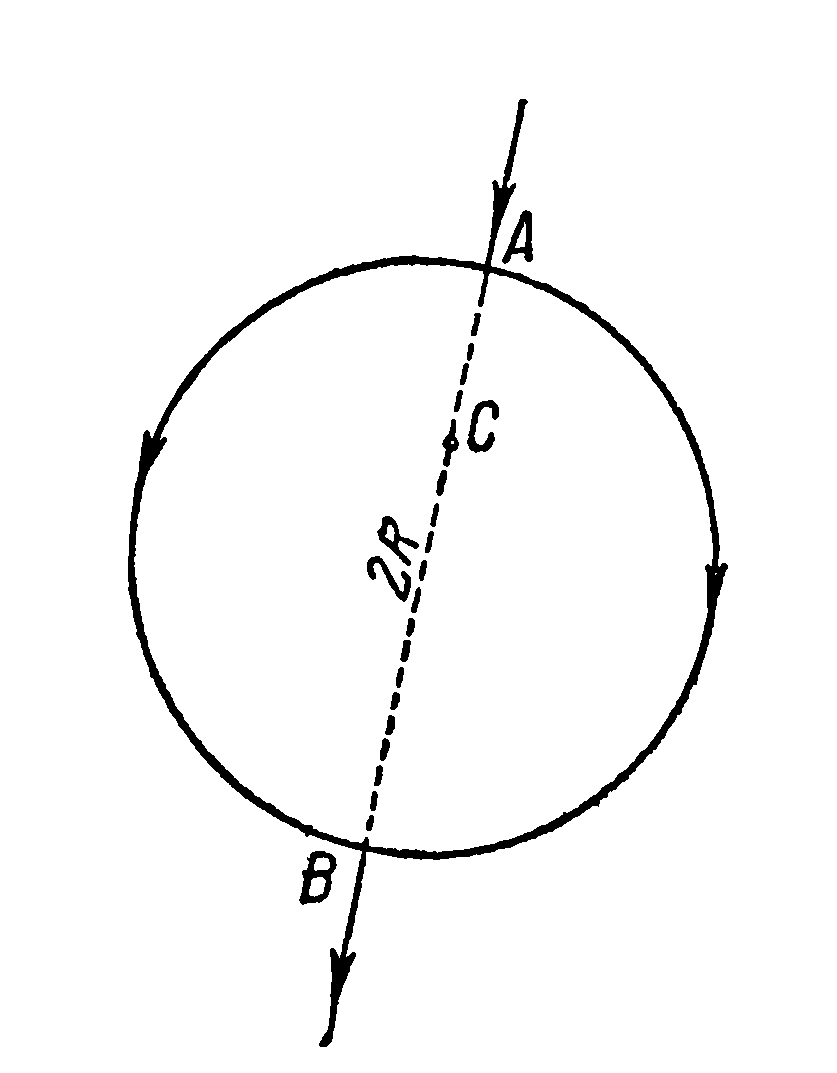
\includegraphics[width=0.4\linewidth]{task_pic}
	\label{task_pic}
	\caption{Контур}
\end{figure}

Две полуокружности можно представить как две одинаковых параллельных ветви с одинаковым сопротивлением.
Значит величина тока будет одна и таже, а направление противоположное. Поэтому суммарный вектор магнитной
индукции в любой точке диаметра будет равен нулю, а следовательно и вектор ($ Н $) будет равен нулю.

\begin{equation}
	H = 0
\end{equation}
